% \documentclass[handout]{beamer}
%\documentclass[notes]{beamer}
\documentclass{beamer}
\errorcontextlines 10000
%\usepackage{pgfpages}
%\setbeamertemplate{note page}[compress] % default/compress/plain
%\setbeameroption{show notes on second screen=right}


\batchmode
\graphicspath{ {./figures/} }


\usetheme[greybg]{sthlm}
\setbeamercovered{dynamic}
\setbeamertemplate{navigation symbols}{}%remove navigation symbols
\setbeamertemplate{blocks}[rounded][shadow=false]
\setbeamertemplate{headline}{%
  \leavevmode%
  \begin{beamercolorbox}[colsep=1.5pt]{upper separation line head}
  \end{beamercolorbox}
  \begin{beamercolorbox}{section in head/foot}
    \vskip2pt\insertnavigation{\paperwidth}\vskip2pt
  \end{beamercolorbox}%
  \begin{beamercolorbox}[colsep=10.5pt]{lower separation line head}
  \end{beamercolorbox}
}
\setbeamertemplate{footline}
{%
  \leavevmode%
  \hbox{\begin{beamercolorbox}[wd=.5\paperwidth,ht=2.5ex,dp=1.125ex,leftskip=.3cm plus1fill,rightskip=.3cm]{author in head/foot}%
      \usebeamerfont{author in head/foot}\centering\insertshortauthor
    \end{beamercolorbox}%
    \begin{beamercolorbox}[wd=.5\paperwidth,ht=2.5ex,dp=1.125ex,leftskip=.3cm,rightskip=.3cm plus1fil]{title in head/foot}%
      \usebeamerfont{title in head/foot}\hfill\insertframenumber/\inserttotalframenumber\hspace{2em}
    \end{beamercolorbox}}%
  \vskip0pt%
}



\usepackage[shortlabels]{enumitem}
\setlist{itemsep=0.2cm}
\setlist[itemize]{label={\tiny$\color{issrBlue!30!white}\blacktriangleright$}}
\setlist[itemize,1]{itemsep=0.5cm}
\setlist[enumerate]{label={\small\protect\color{issrBlue!50!white}\arabic*.}}
\setlist[description]{font=\color{issrBlue}}

\newcommand{\compresslist}{%
  \setlength{\itemsep}{0em}%
  \setlength{\parskip}{0pt}%
  \setlength{\parsep}{0pt}%
}

\usepackage[utf8]{inputenc}


\renewcommand*{\familydefault}{\sfdefault}
\def\tt{\normalfont\ttfamily}

\usepackage[sorting=none,backend=bibtex,autocite=footnote]{biblatex}

\bibliography{references}

\usepackage{multirow}
\usepackage{rotating}
\usepackage{xifthen}

\usepackage{relsize}
\usepackage{soul}
\usepackage{cancel}

\usepackage{amsmath}
\usepackage{amsfonts}
\usepackage{amsthm}
\usepackage{bm}
\newcommand*\circled[1]{%
  \tikz[baseline=(char.base)]{%
    \node[circle,draw=none,inner sep=0pt,minimum height=1em] (char) {#1};
    \draw (char) circle (0.55em);
  }}

\newcommand{\fn}[1]{\bm{\mathit{#1}}}
\newcommand{\angledlist}[1]{\langle #1 \rangle}
\newcommand{\pr}[1]{\mbox{Pr}(#1)}

% Staccato
\newcommand{\bigO}[1]{\fn{\mathcal O}\big(#1\big)}
\newcommand{\powSet}[1]{\fn{\mathcal P}(#1)}

\newcommand{\staccato}{\textit{Staccato}}
\newcommand{\mhsII}{\texorpdfstring{$\textit{MHS}^\text{\smaller2}$}{MHS2}}
\renewcommand{\mhsII}{$MHS^\text{\smaller2}$}
\newcommand{\mhsIIURL}{\url{https://github.com/npcardoso/MHS2}}

\newcommand{\HS}{\fn{HS}}
\newcommand{\MHS}{\fn{MHS}}

\newcommand{\setupName}[1]{\textit{#1}}
\newcommand{\Opt}[1]{\setupName{Opt $\mathit{#1}$}}
\newcommand{\Opts}[2]{\setupName{Opts $\mathit{#1}$ -- $\mathit{#2}$}}


% Fuzzinel
\newcommand{\cerror}[1][F]{\fn{\mu_{#1}}}
\newcommand{\ferror}[1][F]{\fn{\mu_{\widetilde{#1}}}}
\newcommand{\fuzzinel}{\texorpdfstring{$\textit{Fuzzinel}$}{Fuzzinel}}
\newcommand{\likelihoodii}[2][d]{\pr{A_{#2},e_{#2}\mid #1}}
\newcommand{\likelihoodi}[1][d]{\pr{A_i,e_i\mid #1}}
\newcommand{\likelihood}[1][d]{\pr{A,e\mid #1}}
\newcommand{\prior}[1][d]{\pr{#1}}
\newcommand{\posterior}[1][d]{\pr{#1\mid A,e}}
\newcommand{\gFunc}[1][d]{\fn{G}(#1, A_i)}
\providecommand{\e}[1]{\ensuremath{\times 10^{#1}}}

\newcommand{\likelihoodcii}[2][d]{\pr{A_{#2},e_{#2},c_{#2}\mid #1}}
\newcommand{\likelihoodci}[1][d]{\pr{A_i,e_i,c_i\mid #1}}
\newcommand{\likelihoodc}[1][d]{\pr{A,e,c\mid #1}}
\newcommand{\posteriorc}[1][d]{\pr{#1\mid A,e,c}}

% NFGE
\newcommand{\BW}{\mathit{bw}}
\newcommand{\ST}{\mathit{st}}
\newcommand{\FB}{\mathit{FB}}
\newcommand{\KDEfunc}[1][ej]{\fn{pdf_{#1}}}
\newcommand{\KDE}[1][ej]{\KDEfunc[#1](\ST)}
% \newcommand{\NFGE}{\texorpdfstring{$\textit{NFGE}$}{NFGE}}
\newcommand{\NFGE}{NFGE}
\newcommand{\supergjcomb}[1][j]{\fn{g^+_{#1}}(\ST)}
\newcommand{\supergjcall}[2][\ST]{\texorpdfstring{\fn{\breve{g}_{#2}}(#1)}{g#2(#1)}}
\newcommand{\supergj}[1][j]{\supergjcall{#1}}


\newcommand{\supergFunc}[1][j,S]{\fn{\breve{G}}(#1)}

\newcommand{\etc}{\emph{etc.}}
\newcommand{\ie}{\emph{i.e.}}
\newcommand{\eg}{\emph{e.g.}}
\newcommand{\vs}{\textit{vs.}}



\usepackage{multirow}


\usepackage{color, colortbl}
\setlength{\tabcolsep}{8pt}
\definecolor{Gray}{gray}{0.5}
\definecolor{limegreen}{rgb}{0.5,0.7,0}
\definecolor{lightred}{rgb}{1,0.2,0.2}
\definecolor{lightgreen}{rgb}{0.2,1,0.2}
\colorlet{highlight}{teal!25!white}
\newcolumntype{n}{C{1.6em}}
\newcolumntype{g}{C{1.6em}}

\usepackage{subfig,caption}
\usepackage{float}

\usepackage{tikz,pgfplots}
\usetikzlibrary{matrix}
\usetikzlibrary{chains,matrix,scopes}
\usetikzlibrary{positioning}
\usetikzlibrary{arrows}
\usetikzlibrary{fit}
\usetikzlibrary{shapes,snakes}
\usetikzlibrary{decorations.markings}
\usepgfplotslibrary{groupplots}
\usepgfplotslibrary{fillbetween}
\tikzset{
  >=stealth',
  invisible/.style={opacity=0.1},
  visible on/.style={alt=#1{}{invisible}},
  alt/.code args={<#1>#2#3}{%
    \alt<#1>{\pgfkeysalso{#2}}{\pgfkeysalso{#3}} % \pgfkeysalso doesn't change the path
  },
}
\pgfdeclarelayer{background}
\pgfdeclarelayer{foreground}
\pgfsetlayers{background,main,foreground}


\newcommand\cthit{\circled{$\bm{\times}$}}
\newcommand\chit{\circled{\checkmark}}
\newcommand\hit{$\bullet$}
\newcommand\nhit{.}



\newcommand{\citep}{}
\newcommand{\ac}[1]{#1}
\newcommand{\acl}[1]{#1}


\colorlet{clra}{teal}
\colorlet{clrb}{orange!80!white}
\colorlet{clrc}{cyan}
\colorlet{clrd}{lime}
\colorlet{clre}{red!60!white}
\colorlet{dkclra}{clra!50!black}
\colorlet{dkclrb}{clrb!90!black}
\colorlet{dkclrc}{clrc!50!black}
\colorlet{dkclrd}{clrd!50!black}
\colorlet{dkclre}{clre!60!white!80!black}

%%%%%%%%%%%%%%%%%%%%%%%%%%%%%%%%%%%%%%%%%%%%%%%%%%%%%%%%%%%%%%%%%%%%%%%%%%%%%%%
%%%%%%%%%%%%%%%%%%%%%%%%%%%%% Notes page%%%%%%%%%%%%%%%%%%%%%%%%%%%%%%%%%%%%%%%
%%%%%%%%%%%%%%%%%%%%%%%%%%%%%%%%%%%%%%%%%%%%%%%%%%%%%%%%%%%%%%%%%%%%%%%%%%%%%%%

\makeatletter
\defbeamertemplate{note page}{infolines}
{%
  \hspace{-0.6cm}%
  \vbox{%
    \hbox{%
      \begin{columns}%
        \column{\dimexpr\paperwidth-10pt}%
        \bicolumn{%
          \vspace{-1cm}%
          \insertslideintonotes{0.5}%
        }{%
          \displaytargettime%
        }
        \LARGE%
        \insertnote%
      \end{columns}
    }%
  }%
}
\makeatother


\setbeamertemplate{note page}[infolines]

\newcommand{\lasttargettime}{0 min}
\newcommand{\targettime}{0 min}
\newcommand{\settargettime}[1]{
  \edef\x{\targettime}
  \renewcommand{\lasttargettime}{\x}
  \renewcommand{\targettime}{#1}
}


\newcommand{\displaytargettime}{%
  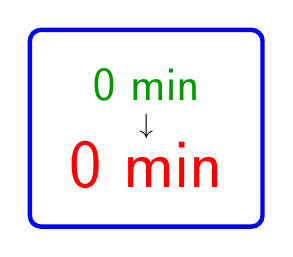
\begin{tikzpicture}
    \node{};
    \node[anchor=north,align=center,draw=blue, ultra thick, rounded corners,inner sep=5mm,fill=white] at (0,0.5cm){
      \color{black!40!green}\LARGE\lasttargettime \\
      $\downarrow$ \\
      \color{red}\Huge\targettime};
  \end{tikzpicture}
}

\newenvironment{slideHeader}{
  \vspace{1em}
  %	\fbox{
  \begin{minipage}[b][5em][t]{\textwidth}
    % }
  }{\end{minipage}}

\newcommand{\centeredExample}[4]{
  \begin{example}
    #1
    \begin{columns}
      \column{0.5\textwidth}
      \begin{center}
        #2
      \end{center}
      \column{0.5\textwidth}
      \begin{center}
        #3
      \end{center}
    \end{columns}
    #4
  \end{example}
}

\usepackage{adjustbox}
\newcommand{\drawaxes}[1]{
  \begin{pgfonlayer}{foreground}
    \draw[->,>=stealth, thick,black] (#1.south west) -- (#1.south east) -> +(0.2cm,0);
    \draw[->,>=stealth, thick,black] (#1.south west) -- (#1.north west) -> +(0,0.2cm);
  \end{pgfonlayer}
}
\newenvironment{tikzbenchmarkfig}[2][]{
  \centering
  \begin{tikzpicture}%
    \tikzstyle{every node}=[node distance=0pt,line width=0.1mm,anchor=north, inner sep=0pt,font=\scriptsize\mdseries,text centered,align=center,#1,black];
    \tikzstyle{main plot}=[fill=none,draw=none]
  }{%
    \drawaxes{main}
  \end{tikzpicture}%
}
\newcommand{\scaleig}[2][scale=0.7]{\includegraphics[#1]{#2}}
\colorlet{bggray}{white!99!black}




\tikzstyle{inner box} = [box, clip]
\tikzstyle{outer box} = [fill=none,box, thick, draw]
\tikzstyle{box} = [inner sep=0pt,outer sep=0pt, rounded corners]
\tikzstyle{line} = [draw,rounded corners, -latex',ultra thick]



\begin{document}
\section{Introduction}
% Define block styles
\tikzstyle{defaults} = [text badly centered, draw, font=\Large,inner sep=5mm]
\tikzstyle{decision} = [defaults, diamond, fill=clra, text width=4.5em,  node distance=3cm, inner sep=0pt]
\tikzstyle{block} = [defaults, rectangle, fill=clrb, text width=7cm, rounded corners, minimum height=2cm]
\tikzstyle{line} = [draw,rounded corners=5pt, -latex',ultra thick]
\tikzstyle{cloud} = [defaults,text width=10em,rectangle,fill=clrc, node distance=3cm, minimum height=3em]


\settargettime{3 min}
\subsection{Context}
\frameready{}{
  \begin{frame}
  \frametitle{Context}
  \framesubtitle{Motivation}
  \monocolumn{
    \begin{itemize}
    \item Despite the advances made in the Computer Science domain, it
      remains practically \alert{impossible to create faultless systems}
    \end{itemize}
  }
  \note{
    \begin{itemize}
    \item A motivação geral...
    \item chegam a \alert{estadios de prod} com defeitos...
    \end{itemize}

  }
\end{frame}

  \begin{frame}
  \frametitle{Context}
  \framesubtitle{Self-healing Systems}
  \monocolumn{
    \begin{itemize}
    \item Research in \alert{Self-healing Systems} aims at:
      \begin{enumerate}
        \setlength{\itemsep}{0pt}
      \item Improving the systems' dependability
      \item Reducing human intervention
      \end{enumerate}
    \end{itemize}
    \vspace{2em}
    \resizebox{0.4\columnwidth}{!}{
      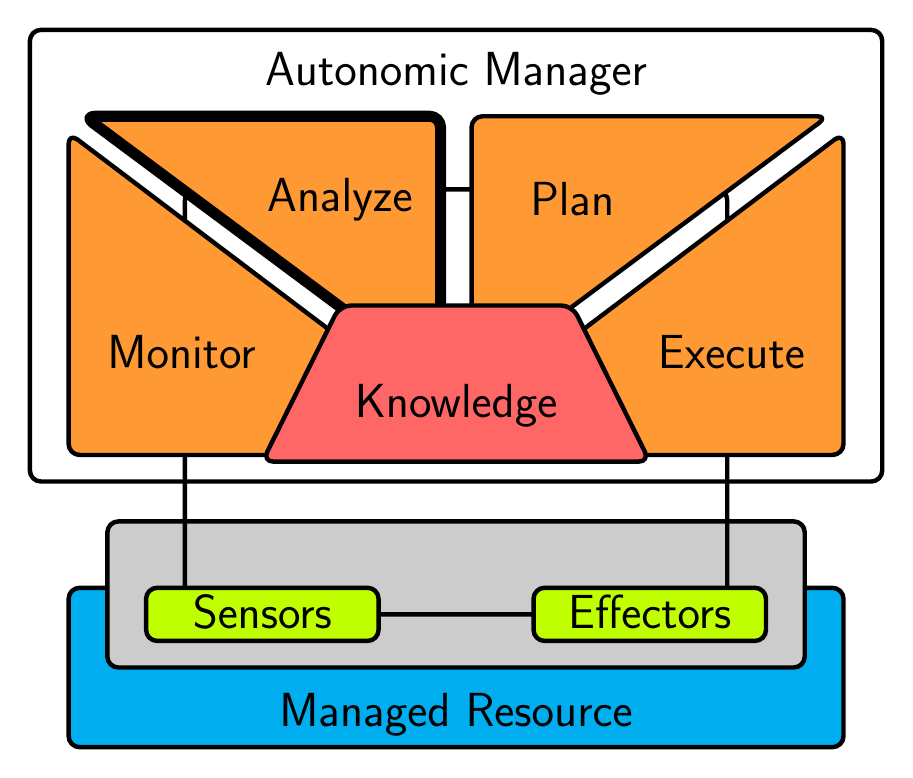
\begin{tikzpicture}[y=0.80pt, x=0.8pt, inner sep=0pt, outer sep=0pt,yscale=-1,font=\LARGE]
        \tikzstyle{ll}=[draw=black,line join=round,line cap=butt,miter
        limit=4,nonzero rule,ultra thick,rounded corners];

        \tikzstyle{aw}=[anchor=west];
        \tikzstyle{ae}=[anchor=east];
        \tikzstyle{ac}=[anchor=center];


        \begin{scope}[xscale=1.4,yscale=1.5]

          \begin{scope}[yshift=100,xscale=250,yscale=40]
            \path[ll,fill=clrc] (0,1) rectangle (1,2.2);
            \draw[ll,fill=white!80!black] (0.05,0.5) rectangle (0.95,1.6);
            \path[ll,fill=white] (-0.05,0.2) rectangle (1.05,-3.2);
            \path[ll] (0.15,-2) rectangle (0.85,1.2);
            \path[ll,fill=clrd] (0.1,1) rectangle (0.4,1.4);
            \path[ll,fill=clrd] (0.6,1) rectangle (0.9,1.4);
          \end{scope}

          \begin{scope}[xshift=0,xscale=250]
            \path[ll,fill=clrb] (0.3,125) -- (0,125) -- (0,28) -- (0.38,95) --  cycle;
            \path[ll,fill=clrb,line width=4pt] (0.02,23) -- (0.4,89) -- (0.48,89) -- (0.48,23)  -- cycle;
            \path[ll,fill=clrb] (0.98,23) -- (0.6,89) -- (0.52,89) -- (0.52,23)  -- cycle;
            \path[ll,fill=clrb] (1,125) -- (1,28) -- (0.62,95) -- (0.62,125) -- cycle;
            \path[ll,fill=clre] (0.25,127) -- (0.35,80) -- (0.65,80) -- (0.75,127) -- cycle;


            \begin{scope}[yshift=20, yscale=230]
              \path(0.5,-0.065) node {Autonomic Manager};
              \path[ac](0.25,0.64) node {Sensors};
              \path[ac](0.75,0.64) node {Effectors};
              \path(0.5,0.775) node {Managed Resource};
              \path[aw] (0.05,0.3) node {Monitor};
              \path(0.35,0.1) node {Analyze};
              \path(0.65,0.1) node {Plan};
              \path[ae] (0.95,0.3) node {Execute};
              \path(0.5,0.37) node {Knowledge};
            \end{scope}
          \end{scope}
        \end{scope}
      \end{tikzpicture}
    }
  }
  \note{
    \begin{itemize}
    \item \alert{Como resposta a este problema} ....
    \item Em contraste... \alert{automatismos que permitam}
    \item As contribuições inserem-se na fase de analise
    \end{itemize}

  }
\end{frame}

  \begin{frame}[c]
  \frametitle{Context}
  \framesubtitle{Diagnostic Problem}
  \monocolumn{
    \begin{itemize}
    \item A \alert{diagnostic problem} occurs whenever the behavior
      of a particular system \alert{deviates} from the
      \alert{expected behavior}
    \item The challenge is to find the \alert{true root causes} of
      the \alert{abnormal behavior}
    \end{itemize}
  }
\end{frame}

}

\settargettime{5 min}
\subsection{Spectrum-based Fault Localization}
\frameready{}{
  \begin{frame}
  \frametitle{Spectrum-based Fault Localization}
  \framesubtitle{Abstraction}

  \monocolumn{%
    \begin{description}
    \item [\alert{Component} --] An indivisible\footnotemark[1] element of the system
    \item [\alert{Transaction} --] A set of \alert{component} activations that:
      \begin{enumerate}
      \item Share a \alert{common goal}
      \item The \alert{correctness} of the output can be \alert{verified}
      \end{enumerate}
    \end{description}
  }%

  \footnotetext[1]{From a diagnosis point-of-view}

  \note{
    \begin{itemize}
    \item Reasoning Based SFL
    \item \alert{$\uparrow$ Precisão}/\alert{$\downarrow$ complexidade}$\Rightarrow$abst de alto nível
    \item Verificar se o resultado \alert{foi o esperado}
    \end{itemize}


  }
\end{frame}

  \begin{frame}
  \frametitle{Spectrum-based Fault Localization}
  \framesubtitle{Spectrum}
    \monocolumn{%
      \begin{description}
      \item [\alert{Spectrum} --] A pair $(A, e)$ encoding:
        \begin{description}
        \item[\alert{$A_{ij}$} --] \alert{Activity} of component $j$ in transaction $i$
        \item[\alert{$e_i$} --] \alert{Error} state of transaction $i$ (pass/fail)
        \end{description}
      \end{description}
    }%

  \vfill%
  \vfill%

  \monocolumn{%
    \begin{tikzpicture}[
      act/.style = {fill=clrc,ultra thick},
      inact/.style = {fill=white!80!black,thick},
      pass/.style = {fill=clrd},
      fail/.style = {fill=clre},
      cmp/.style = {circle, draw, align=center,minimum size=1.5em,inner sep=0.1cm,anchor=center},
      tr/.style = {draw,box,thick, minimum width=4cm, inner sep = 0.5cm}]

      \setlength{\tabcolsep}{0pt}%
      \renewcommand{\arraystretch}{1.2}%


      \node[inner box] (a){%
        \begin{tabular}[m]{C{1cm}|*{3}{C{1cm}}|C{1cm}C{0cm}}
          \multirow{2}{*}{$i$} & \multicolumn{3}{c|}{$A_{ij}$} & \multirow{2}{*}{$e_i$}                                          \\\cline{2-4}
                               & $c_1$                    & $c_2$             & $c_3$             &                       \\\hline%
          \onslide<2->{ $1$     & \cellcolor{clrc}1        & \cellcolor{clrc}1 & 0                 & \cellcolor{clre}1  &\\}
          \onslide<3->{$2$     & \cellcolor{clrc}1        & 0                 & \cellcolor{clrc}1 & \cellcolor{clre}1  &\\}
          \onslide<4->{$3$     & \cellcolor{clrc}1        & 0                 & 0                 & \cellcolor{clrd}0  &}
        \end{tabular}%
      };
      \node[outer box,fit=(a)] {};


      \foreach \id /\ca / \cb / \cc / \res in {
        0/inact/inact/inact/,
        1/act/act/inact/fail,
        2/act/inact/act/fail,
        3/act/inact/inact/pass} {
        \pgfmathparse{int(\id+1)}
        \edef\slideId{\pgfmathresult}
        \only<\slideId>{
          \node[\res,tr,left= of a.west] (transaction){};
          \node[\ca,cmp,right=0.5cm of transaction.west]  {$c_1$};
          \node[\cb,cmp] at (transaction) {$c_2$};
          \node[\cc,cmp,left=0.5cm of transaction.east] {$c_3$};
        }
      }

    \end{tikzpicture}
  }%
  \note{
    \begin{itemize}
    \item \alert{Sistema de armazenamento de dados}
    \end{itemize}
  }
\end{frame}

  \begin{frame}
  \frametitle{Spectrum-based Fault Localization}
  \framesubtitle{Workflow}
  \monocolumn{
    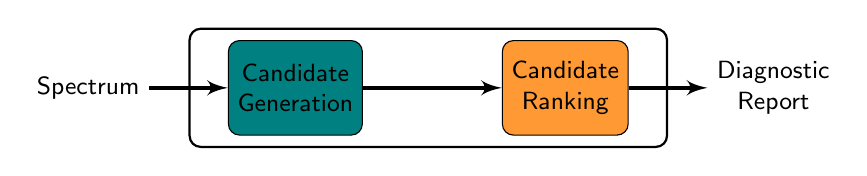
\begin{tikzpicture}
      \tikzstyle{every node}=[
      align=center,
      minimum height=1.2cm,
      font=\small];

      \node [rectangle, rounded corners, draw, anchor=north, minimum width=0.5\columnwidth,fill=white,thick,    minimum height=1.5cm,
      ] (box) at (0, 0){};


      \node [left=0.5cm of box] (obs) {Spectrum};
      \node [right=0.5cm of box] (diag){Diagnostic \\ Report};


      \node [fill=clra,rectangle, rounded corners, draw, left = -0.5cm of box, anchor=west] (cg) {Candidate \\ Generation};
      \node [fill=clrb,rectangle, rounded corners, draw, right = -0.5cm of box, anchor=east] (cr) {Candidate \\ Ranking};
      \path[line] (obs.east) --(cg);
      \path[line] (cg) -> (cr);
      \path[line] (cr) -- (diag.west);
    \end{tikzpicture}%
  }
  \vfill
  \monocolumn{
    \begin{enumerate}
    \item Generate possible \alert{explanations for the erroneous behavior}
    \item Minimize the number of \alert{unnecessarily  inspected}  components
    \end{enumerate}
  }
  \note{
    \begin{itemize}
    \item \alert{Relatório de diagnóstico}
    \end{itemize}


  }

\end{frame}

}

\settargettime{10 min}
\subsection{Candidate Generation}
\frameready{}{
  \begin{frame}
  \frametitle{Candidate Generation}
  \framesubtitle{Diagnostic Candidate}
  \only<1>{
    \monocolumn{
      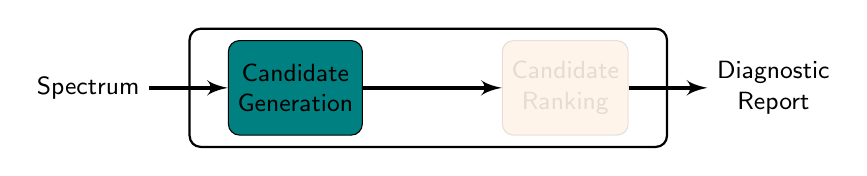
\begin{tikzpicture}
        \tikzstyle{every node}=[
        align=center,
        minimum height=1.2cm,
        font=\small];
        \node [rectangle, rounded corners, draw, anchor=north, minimum width=0.5\columnwidth,fill=white,thick,    minimum height=1.5cm,
        ] (box) at (0, 0){};


        \node [left=0.5cm of box] (obs) {Spectrum};
        \node [right=0.5cm of box] (diag){Diagnostic \\ Report};


        \node [fill=clra,rectangle, rounded corners, draw, left = -0.5cm of box, anchor=west] (cg) {Candidate \\ Generation};
        \node [opacity=0.1,fill=clrb,rectangle, rounded corners, draw, right = -0.5cm of box, anchor=east] (cr) {Candidate \\ Ranking};
        \path[line] (obs.east) --(cg);
        \path[line] (cg) -> (cr);
        \path[line] (cr) -- (diag.west);
      \end{tikzpicture}%

      \vspace{1em}

      \begin{description}
      \item [Candidate] Every failed transaction activates at least
        one faulty component
      \item [Minimal] No smaller subset of components meets the above
        criterion
      \end{description}
    }
  }

  \only<2>{
  \monocolumn{
      \resizebox{!}{5cm}{
        \begin{tikzpicture}[->=latex]
          \setlength{\tabcolsep}{0pt}%
          \renewcommand{\arraystretch}{1.2}%
          \tikzstyle{line} = [draw,rounded corners, -latex',ultra thick]
          \tikzstyle{box} = [inner sep=0pt,outer sep=0pt, rounded corners]
          \tikzstyle{inner box} = [box, clip]
          \tikzstyle{outer box} = [box, thick, draw]

          \node[inner box] (a){
            \begin{tabular}[m]{*{3}{C{1cm}}|C{1cm}C{0cm}}
              {$c_1$} & $c_2$ & $c_3$ & $e_i$             \\\hline%
              \hit    & \hit  & \nhit & \cellcolor{clre}1 \\
              \hit    & \nhit & \hit  & \cellcolor{clre}1 \\\hline
              \hit    & \nhit & \nhit & \cellcolor{clrd}0
            \end{tabular}%
          };
          \node[outer box,fit=(a)] {};

          \node[inner box, right= of a] (b) {%
            \begin{tabular}[m]{*{3}{C{1cm}}}
              $c_1$ & $c_2$ & $c_3$ \\\hline%
              \hit  & \hit  & \nhit \\
              \hit  & \nhit & \hit
            \end{tabular}%
          };
          \node[outer box,fit=(b)] {};

          \node[anchor=north,inner box,below=of b.south] (d) {%
            \begin{tabular}[m]{*{3}{C{1cm}}}%
              $c_1$ & \cellcolor{clra}$c_2$ & \cellcolor{clra} $c_3$ \\\hline%
              \hit  & \chit                 & \nhit                  \\
              \hit  & \nhit                 & \chit
            \end{tabular}%
          };
          \node[outer box,fit=(d)] {};

          \node[anchor=north east,inner box, below left=0cm and 1cm  of d.north west] (c) {%
            \begin{tabular}[m]{*{3}{C{1cm}}}%
              \cellcolor{clra}$c_1$ & $c_2$ & $c_3$ \\\hline%
              \chit                 & \hit  & \nhit \\
              \chit                 & \nhit & \hit
            \end{tabular}%
          };
          \node[outer box,fit=(c)] {};

          \node[anchor=north west,inner box,below right=0cm and 1cm of d.north east] (e) {%
            \begin{tabular}[m]{*{3}{C{1cm}}}%
              \cellcolor{clrb}$c_1$ & \cellcolor{clrb}$c_2$ & \cellcolor{clrb} $c_3$ \\\hline%
              \cthit                & \cthit                & \nhit                  \\
              \cthit                & \nhit                 & \cthit
            \end{tabular}%
          };
          \node[outer box,fit=(e)] {};

          \draw[line] (a) -> (b);
          \draw[line] (b) -> (c);
          \draw[line] (b) -> (d);
          \draw[line] (b) -> (e);
        \end{tikzpicture}
      }
    }
  }
  \note{
    \begin{itemize}
      \LARGE
    \item \alert{Conceitos importantes}
    \end{itemize}
  }
\end{frame}

  % Define block styles
\tikzstyle{decision} = [diamond, draw, fill=clra,
text width=4.5em, text badly centered, node distance=3cm, inner sep=0pt]
\tikzstyle{block} = [rectangle, draw, fill=clrb,
text width=8em, text centered, rounded corners, minimum height=4em]
\tikzstyle{line} = [draw,rounded corners=5pt, -latex',ultra thick]
\tikzstyle{cloud} = [text badly centered,text width=8em,draw, rectangle,fill=clrc, node distance=3cm,
minimum height=2em]

\tikzstyle{decision label} = [text badly centered,anchor=center,near start,fill=white,draw=black,font=\small,execute at begin node={\begin{varwidth}{5em}},
  execute at end node={\end{varwidth}}]
\begin{frame}
  \frametitle{Candidate Generation}
  \framesubtitle{Algorithm}
  \pgfdeclarelayer{background}
  \pgfsetlayers{background,main}
  \monocolumn{
    \resizebox{\columnwidth}{!}{
      \begin{tikzpicture}[>=latex,node distance = 2cm, auto]
        % Place nodes
        \node [cloud] (ft) {$S$ (failed tr.)};
        \node [cloud, below=1cm of ft] (d) {$d$ (current set)};
        \node [cloud, below=1cm of d] (D) {$D$ (candidate set)};
        \begin{pgfonlayer}{background}
          \node[inner sep=0.5cm,thick,draw,dotted,fit=(d.north west) (D.south east), fill=clrc,fill opacity=0.4] (default args) {};
        \end{pgfonlayer}
        \node [anchor=north,below = 0cm of default args.south]{Initially empty};

        \onslide<+(1)->{
          \node [decision, right= 2cm of d] (empty) {is $S$ empty?};
          \path [line] (ft.east) -| +(1,-0.5)  |- (empty.west);
          \path [line] (d.east) -- (empty.west);
          \path [line] (D.east)  -| +(1, 0.5)  |- (empty.west);
        }

        \onslide<+(1)->{
          \node [block, below right= 0.5cm and 10cm of empty.east] (return) {Return $D$};

          \node [decision, above right= 2cm and 1cm of empty] (minimal) {is $d$ minimal?};
          \path [line] (empty.north) -- +(0,0.5)  |-node [decision label] {\textbf{yes}: $d$ is a candidate}(minimal.west);
          \path [line] (minimal.south) |- node [decision label] {\textbf{no}}(return.west);

          \node [anchor=west, block, right= 2.5cm of minimal.east] (purge) {remove super-sets of $d$ from $D$};
          \path [line] (minimal.east) -- node [decision label,midway] {\textbf{yes}}(purge.west);

          \node [block] (add) at (return |- purge) {add $d$ to $D$};
          \path [line] (purge.east) --   (add.west);
          \path [line] (add.south) -- (return.north);
        }

        \onslide<+(1)->{
          \coordinate [below = 2cm of empty] (sort) {};
          \path [line,-] (empty.south) --  node [decision label,midway] {\textbf{no}: $d$ is not a candidate} (sort.north);

          \node [block, below= 1cm of sort] (filter) {create temporary $S'$ filtering transactions where $c$ is active};

          \node [block, right = 1cm of filter] (call) {recursive call with $S'$, $d\cup\set{c}$};
          \path [line] (filter.east) --   (call.west);

          \node [block, right= 1cm of call] (update) {update $D$ with return value};
          \path [line] (call.east) -- (update.west);

          \begin{pgfonlayer}{background}
            \node[inner sep=0.5cm,thick,draw,dotted,fit=(filter.north west) (update.south east), fill=clrb,fill opacity=0.4] (loop) {};
          \end{pgfonlayer}

          \node [anchor=south,above = 0cm of loop.north]{For each component $c$};
          \draw [fill=black] (loop.west) circle (0.2cm);
          \draw [fill=black] (loop.east) circle (0.2cm);


          \path [line] (sort.south) |-  +(-3,-0.25) |- ($(loop.west)+(-0.2cm,0)$);
          \path [line]  ($(loop.east)+(+0.2cm,0)$) -| (return.south);

        \end{tikzpicture}
      }
    }
  }
  \note{
    \begin{itemize}
      \LARGE
    \item \alert{Conjunto} d
    \item \alert{Lista de candidatos} D
    \end{itemize}
  }
\end{frame}

  \newcommand{\rhit}{\rowcolor{clra}}
\newcommand{\hhit}[1]{\cellcolor{clrb}$#1$}
\newcommand{\staccatospectracall}[2]{%
  \begin{tabular}[b]{#1}
    #2
  \end{tabular}%
}

\tikzset{
  vis/.style={visible on=<#1->},
  mcand/.style={line width=5pt},
  cand/.style={alt=<#1->{}{mcand}},
}
\tikzstyle{line} = [draw,rounded corners, -latex',ultra thick]

\begin{frame}
  \frametitle{Candidate Generation}
  \framesubtitle{Example}
  \monocolumn{
    \resizebox{\columnwidth}{!}{
      \begin{tikzpicture}[thick]
        \tikzstyle{every node}=[fill=white,node distance=1.5cm, anchor=west, align=left, rounded corners, draw, inner sep=2pt]

        \setlength{\tabcolsep}{6pt}

        \node (a0) {
          \staccatospectracall{nnn}
          {$c_1$ & $c_2$ & $c_3$ \\ \hline
            \hit  & \hit   & \nhit   \\
            \hit  & \nhit   & \hit   \\}};

        \node[align=center,mcand,above left=1cm and 3cm of a0.west,inner sep=1em](xxxx)  {Minimal \\ Candidate};

        \node[left=1cm of xxxx.west]  {
          \begin{tabular}{cc}
            $c\not\in d$&\cellcolor{clrb} $c\in d$ \\ \hline
            \multicolumn{2}{c}{Unfiltered} \\
            \multicolumn{2}{c}{\cellcolor{clra}Filtered} \\
          \end{tabular}};

        \onslide<3->{
          \node[mcand,below=of a0] (b1) {
            \staccatospectracall{gnn}
            {\hhit{c_1}  & $c_2$ & $c_3$ \\ \hline
              \rhit\chit & \hit  & \nhit \\
              \rhit\chit & \nhit & \hit  \\}};
        }
        \onslide<2->{
          \node[left=3cm of b1] (b0) {
            \staccatospectracall{ngn}
            {$c_1$      & \hhit{c_2} & $c_3$ \\ \hline
              \rhit\hit & \chit      & \nhit \\
              \hit      & \nhit      & \hit  \\}};
        }



        \onslide<2->{
          \node [cand=3,below=of b0.south west](c0) {
            \staccatospectracall{ggn}
            {\hhit{c_1} & \hhit{c_2} & $c_3$ \\ \hline
              \rhit\chit & \chit      & \nhit \\
              \rhit\chit     & \nhit      & \hit  \\}};

          \node[mcand,right=of c0] (c1) {
            \staccatospectracall{ngg}
            {$c_1$      & \hhit{c_2} & \hhit{c_3} \\ \hline
              \rhit\hit & \chit      & \nhit      \\
              \rhit\hit & \nhit      & \chit      \\}};
        }

        \onslide<4->{
          \node[right=3cm of b1] (b2) {
            \staccatospectracall{nng}
            {$c_1$      & $c_2$ & \hhit{c_3} \\ \hline
              \hit      & \hit  & \nhit      \\
              \rhit\hit & \nhit & \chit      \\}};


          \node[cand=0,below=of b2.south east] (c3) {
            \staccatospectracall{ngg}
            {$c_1$      & \hhit{c_2} & \hhit{c_3} \\ \hline
              \rhit\hit & \chit      & \nhit      \\
              \rhit\hit & \nhit      & \chit      \\}};

          \node[cand=0,left =of c3] (c2) {
            \staccatospectracall{gng}
            {\hhit{c_1}  & $c_2$ & \hhit{c_3} \\ \hline
              \rhit\chit & \hit  & \nhit      \\
              \rhit\chit & \nhit & \chit      \\}};
        }



        \onslide<2->{
          \draw (a0.south) --  (b0.north);
          \draw (b0.south) --  (c0.north);
          \draw (b0.south) --  (c1.north);
        }
        \onslide<3->{
          \draw (a0.south) --  (b1.north);
        }

        \onslide<4->{
          \draw (a0.south) --  (b2.north);
          \draw (b2.south) --  (c2.north);
          \draw (b2.south) --  (c2.north);
          \draw (b2.south) --  (c3.north);
        }


      \end{tikzpicture}
    }
  }
  \note{
    \begin{itemize}
    \item Arvore de pesquisa
    \item No $\rightarrow$ chamada ao algoritmo
    \end{itemize}
  }

\end{frame}

}

\settargettime{14 min}
\subsection{Candidate Ranking}
\frameready{}{
  \begin{frame}
  \frametitle{Candidate Ranking}
  \framesubtitle{Diagnostic Report}
  \monocolumn{
    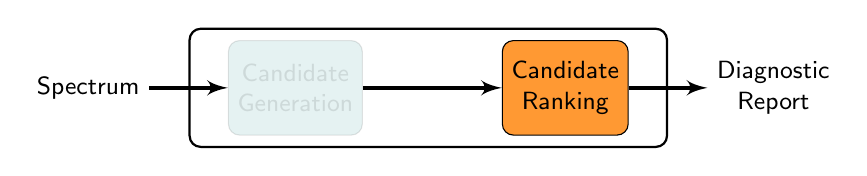
\begin{tikzpicture}
      \tikzstyle{every node}=[
      align=center,
      minimum height=1.2cm,
      font=\small];
      \node [rectangle, rounded corners, draw, anchor=north, minimum width=0.5\columnwidth,fill=white,thick,    minimum height=1.5cm,
      ] (box) at (0, 0){};


      \node [left=0.5cm of box] (obs) {Spectrum};
      \node [right=0.5cm of box] (diag){Diagnostic \\ Report};


      \node [opacity=0.1,fill=clra,rectangle, rounded corners, draw, left = -0.5cm of box, anchor=west] (cg) {Candidate \\ Generation};
      \node [fill=clrb,rectangle, rounded corners, draw, right = -0.5cm of box, anchor=east] (cr) {Candidate \\ Ranking};
      \path [line] (obs.east) --(cg);
      \path [line] (cg) -> (cr);
      \path [line] (cr) -- (diag.west);
    \end{tikzpicture}%

    \vspace{2em}


    \begin{description}
    \item [Intermittent Fault] A fault that is \alert{not consistently triggered} when activated
    \end{description}
  }
  \note{
    \begin{itemize}
    \item \alert{Falha intermitente} quando é ativada \alert{nem
        sempre resulta num erro} (Problema de abstracao!)
    \item \alert{Ex:} função que se propõe a calcular o valor
      \alert{absoluto} de um numero definida como $f(x) = x$
    \end{itemize}
  }
\end{frame}

  \begin{frame}
  \frametitle{Candidate Ranking}
  \framesubtitle{Algorithm}
  \monocolumn{
    \pgfdeclarelayer{background}
    \pgfdeclarelayer{foreground}
    \pgfsetlayers{background,main,foreground}
    \monocolumn{
      \resizebox{\columnwidth}{!}{
        \begin{tikzpicture}[>=latex,node distance = 2cm, auto]
          \onslide<+(1)->{
            \node [block,  anchor=center, minimum height=3.5cm] (bayes) {
              $\pr{d\mid A,e} = $\\[3mm] $\pr{d} \times \displaystyle\prod_{i = 1}^{|A|}\frac{\pr{A_i,e_i \mid d}}{\pr{A_i,e_i}}$\\[5mm]
              (Na\"ive Bayes Classifier)
            };
          }

          \onslide<+(1)->{
            \node [block, below= 1cm of bayes] (goodness) {Estimate goodness parameters \\ (Maximum likelihood estimation)};
            \path [line] (bayes.south)  -- (goodness.north);
          }

          \onslide<+(-2)->{
            \begin{pgfonlayer}{background}
              \node[inner sep=0.5cm,thick,draw,dotted,fit=(bayes.north west) (goodness.south east), fill=clrb,fill opacity=0.4] (loop) {};
            \end{pgfonlayer}
            \node [defaults,draw=none,anchor=south,above = 0cm of loop.north]{For each candidate $d \in D$};
            \begin{pgfonlayer}{foreground}
              \draw [fill=black] (loop.west) circle (0.2cm);
              \draw [fill=black] (loop.east) circle (0.2cm);
            \end{pgfonlayer}
          }

          \node [left=3.8cm of loop.west] (d) {};
          \node [cloud, above=0.4cm of d] (spectrum) {$A, e$ (spectrum)};
          \node [cloud, below=0.4cm of d] (D) {$D$ (candidate set)};

          \onslide<+(-3)->{
            \path [line] (spectrum.east) -| +(0.5,-0.5)  |- ($(loop.west)+(-0.2cm,0)$);
            \path [line] (D.east)  -| +(0.5, 0.5)  |- ($(loop.west)+(-0.2cm,0)$);
          }

          \onslide<+(-1)->{
            \node [block, right=1.5cm of loop.east,text width=3cm] (sort) {Sort $D$};
            \path [line] (loop.east)  -- (sort.west);
          }
        \end{tikzpicture}
      }
    }
  }
  \note{
    \begin{itemize}
      \compresslist
    \item Naive bayes classifier
    \item \alert{Goodness}: Prob de um \alert{COMPONENTE} não gerar um erro
    \item  params incógnitos $\rightarrow$ \alert{MLE}: argmax prob
    \end{itemize}
  }
\end{frame}

  \pgfplotsset{
  cycle list name=exotic,
  axis y line=left,
  axis x line=bottom,
}
\pgfplotsset{%
  colormap={rg}{color(0)=(lime!90!black); color(1)=(red!60!white)},
}

\pgfplotsset{likelihood plot/.style= {
    height=4cm,
    width=0.9\columnwidth,
    samples=40,
    domain=0:1,
    ymin=0,
    xmin=0,
    enlarge y limits=upper,
    every axis plot post/.append style={very thick},
    no markers,
    y tick label style={/pgf/number format/fixed,
      /pgf/number format/1000 sep = \thinspace % Optional if you want to replace comma as the 1000 separator
    },
    z tick label style={/pgf/number format/fixed,
      /pgf/number format/1000 sep = \thinspace % Optional if you want to replace comma as the 1000 separator
    },
  }}

\pgfplotsset{comb/.style= {dashed, draw=gray!40,
    every axis plot post/.append style=
    {mark=*,mark options={fill=lime!90!black,draw=gray!60, solid}} } }

\begin{frame}
  \frametitle{Candidate Ranking}
  \framesubtitle{Example}
  \monocolumn{
    \resizebox{\columnwidth}{!}{
      \begin{tikzpicture}[]
        \setlength{\tabcolsep}{0pt}%
        \renewcommand{\arraystretch}{1.2}%

        \tikzstyle{line} = [draw,rounded corners, -latex',ultra thick]
        \tikzstyle{box} = [inner sep=0pt,outer sep=0pt, rounded corners,align=center]
        \tikzstyle{inner box} = [box, clip]
        \tikzstyle{outer box} = [box, thick, draw]
        \tikzstyle{some space} = [inner sep=0.5em]

        \node[inner box] (a){%
          \begin{tabular}[m]{C{1cm}|*{3}{C{1cm}}|C{1cm}C{0cm}}
            \multirow{2}{*}{$i$} & \multicolumn{3}{c|}{$A_{ij}$} & \multirow{2}{*}{$e_i$}                                          \\\cline{2-4}
                                 & $c_1$                    & $c_2$             & $c_3$             &                       \\\hline%
            $1$     & \cellcolor{clrc}1        & \cellcolor{clrc}1 & 0                 & \cellcolor{clre}1  &\\
            $2$     & \cellcolor{clrc}1        & 0                 & \cellcolor{clrc}1 & \cellcolor{clre}1  &\\
            $3$     & \cellcolor{clrc}1        & 0                 & 0                 & \cellcolor{clrd}0  &
          \end{tabular}};
        \node[outer box,thin,fit=(a)] {};

        \node[inner box, below=of a,some space] (D){%
          $D = \Big\{\set{c_1}, \set{c_2,c_3}\Big\}$
        };

        \node[outer box,fit=(a) (D),some space] (a){};
        \onslide<+(1)->
        {
          \node[inner box, right= of a.east,some space,align=right]  (b){
            $\posterior[\set{c_1}] = \overbrace{ \frac{1}{1000} \cdot \frac{999}{1000} \cdot \frac{999}{1000} }^{\prior} \times \overbrace{\vphantom{\frac{1}{1}} \underbrace{(1-g_1)}_{t_1} \cdot \underbrace{(1-g_1)}_{t_2} \cdot \underbrace{g_1}_{t_3} }^{\likelihood}$
          };
          \node[outer box,fit=(b)] {};

          \draw[line] (a) -> (b);

          \node[outer box,below right= 0.7cm of b.south,some space] (c){
            \begin{tikzpicture}
              \begin{axis} [
                likelihood plot,
                colormap name=rg,
                xlabel={\large$g_1$},
                xtick={0,0.33,0.66,1},
                width=0.45\columnwidth
                ]
                \addplot+[mesh] {(1-x)*(1-x)*(x)};

                \addplot+[ycomb,comb] plot coordinates {(0.333,0.149)};
                \addplot+[xcomb,comb] plot coordinates {(0.333,0.149)};


              \end{axis}
            \end{tikzpicture}
          };
          \draw[line] (b) -> (c);
        }
        \onslide<+(1)->
{
          \node[outer box,below right= of a.south east,some space,anchor=west] (b2){$\posterior[\set{c_2, c_3}] = \cdots$};
          \draw[line] (a) edge[out=0,in=180] (b2);

          \node[outer box,below= 5cm of b.south,some space] (d){
            $\posterior[\set{c_1}] = 0.993$ \\
            $\posterior[\set{c_2,c_3}] = 0.007$
          };
          \draw[line] (b2) ->node[pos=0.5,outer box,some space,fill=white]{$\cdots$} (d);
          \draw[line] (c) -> (d);

        }
      \end{tikzpicture}
    }
  }


  \note{
    \begin{itemize}
      \compresslist
    \item Com este exemplo acabo então a intro da minha apresentação e
      vou  passar a descrever as minhas contribuições.
    \end{itemize}
  }
\end{frame}

}
\note{
  \begin{itemize}
  \item Vou passar agora a apresentar as contribuições feitas no
    ambito do tema que apresentei.
  \end{itemize}
}

\end{document}
